%#MAKEINDEX makeindex interim01
\documentclass[10pt,a4j]{jarticle}

\newcommand{\setcounters}[1] {
  \setcounter{equation}{#1}
  \setcounter{figure}{#1}
  \setcounter{table}{#1}
}

\newcommand{\unit}[1] {
  \hspace{1mm}\mathrm{[#1]}
}

\newcommand{\degc} {
  \hspace{1mm}\mathrm{[}{}^\circ\mathrm{C]}
}

\newcommand{\refig}[1]{図\ref{fig::#1}}
\newcommand{\refeq}[1]{式(\ref{eq::#1})}
\newcommand{\reftab}[1]{表\ref{tab::#1}}

\newcommand{\fig}[5] {
  \begin{figure}[#1]
    \begin{center}
      \includegraphics[width=#2\hsize]{#3}
    \end{center}
    \caption{#4}
    \label{fig::#5}
  \end{figure}
}

\makeatletter
\def\eq{\@ifstar\@eq\@@eq}
\def\@eq#1{\begin{equation*}#1\end{equation*}}
\def\@@eq#1#2{\begin{equation}#2\label{eq::#1}\end{equation}}
\makeatother

\newcommand{\diff}[2] {
  \frac{\mathrm{d}#1}{\mathrm{d}#2}
}

\newcommand{\pdiff}[2] {
  \frac{\partial #1}{\partial #2}
}


\newcommand{\ddt}[2][1] {
  \ifnum #1 < 2
    \frac{\mathrm{d}#2}{\mathrm{d}t}
  \else
    \frac{\mathrm{d}^#1#2}{\mathrm{d}t^#1}
  \fi
}

\newcommand{\e}[1] {
  \mathrm{e}^{#1}
}

\newcommand{\lparen}{(}
\catcode `( = \active
\newcommand{(}{\ifmmode\left\lparen\else\lparen\fi}

\newcommand{\rparen}{)}
\catcode `) = \active
\newcommand{)}{\ifmmode\right\rparen\else\rparen\fi}

\newcommand{\bmat}[1] {
  \begin{bmatrix} #1 \end{bmatrix}
}

\input{include/preamble.tex}


\begin{document}

\begin{titlepage}

  \vspace*{25mm}

  \begin{center}
    {\huge 知能制御PBL\\}
    \vspace{5mm}
    {\Huge 第1回RCR中間報告\\}
    \vspace{20mm}
    {\Large 2017年4月26日}

    \vspace{25mm}

    {\LARGE 西田研究室\\}

    \vspace{10mm}

    {\Large 14104043 桑野僚大\\
   14104034 下松八重宏太\\
   14104090 中尾真人\\
   14104111 本田空\\
   14104131 山崎達也\\
   16104313 山下翔}

  \end{center}

\end{titlepage}



\newpage
\section{目的}
学部3年までに学習した制御理論や電気回路,
情報工学の知識を使って, 競技場内を自律的に走行するロボットカーの製作を行う.
各研究室でチーム一丸となってプロジェクトを進行し,
共同で課題を達成することの難しさや楽しさを学び,
エンジニアとして仕事を進めるための素養を身に付ける.


\section{Robot Car Race(RCR)2017競技ルール}
\subsection{ルール概要}
競技場には黄色のポールや,火災に見立てた複数の赤色のポールが設置されている.
ポールに接触せず,できるだけ速やかに火災を鎮火させる
消防ロボットカー(ロボカー)を作成する.

\subsection{競技場詳細}
競技場の全体図を図\ref{course}に示し,以下に詳細を説明する.
\begin{enumerate}
  \item 競技場は板張りの床であり,縦・横ともに 5400[mm]である.

  \item 競技場には黄色の固定ポールと赤色の火災ポールが設置されており,
        スタートからゴールまで,固定ポールには接触,
        火災ポールには衝突することなく通過しなければならない.

  \item 火災ポールは青色の鎮火ポールに赤色の幕を被せたものであり,
        上部におもり などを落としたり,幕を剥がしたりすることで,
        鎮火ポールに変化させる(このポールの製作も行うこと).

  \item スタート後は右手に固定ポールを見ながら直進し,
        消火活動開始区間まで移動しなければならない.消火活動開始区間に
        進入後は,右折し,火災ポールを発見し次第,消火にあたる.

  \item すべての火災ポールを消火して,鎮火ポールに変化させたのち,
        ゴール地点で停止する.

  \item 火災ポールの配置は競技ごとに異なる.
        また,鎮火ポールが存在することもある.

  \item ポールは直径 80[mm]・高さ 120[mm]の中空パイプであり,
        黄・赤・青の色が付けられている.
\end{enumerate}

\begin{figure}[t]
  \begin{center}
    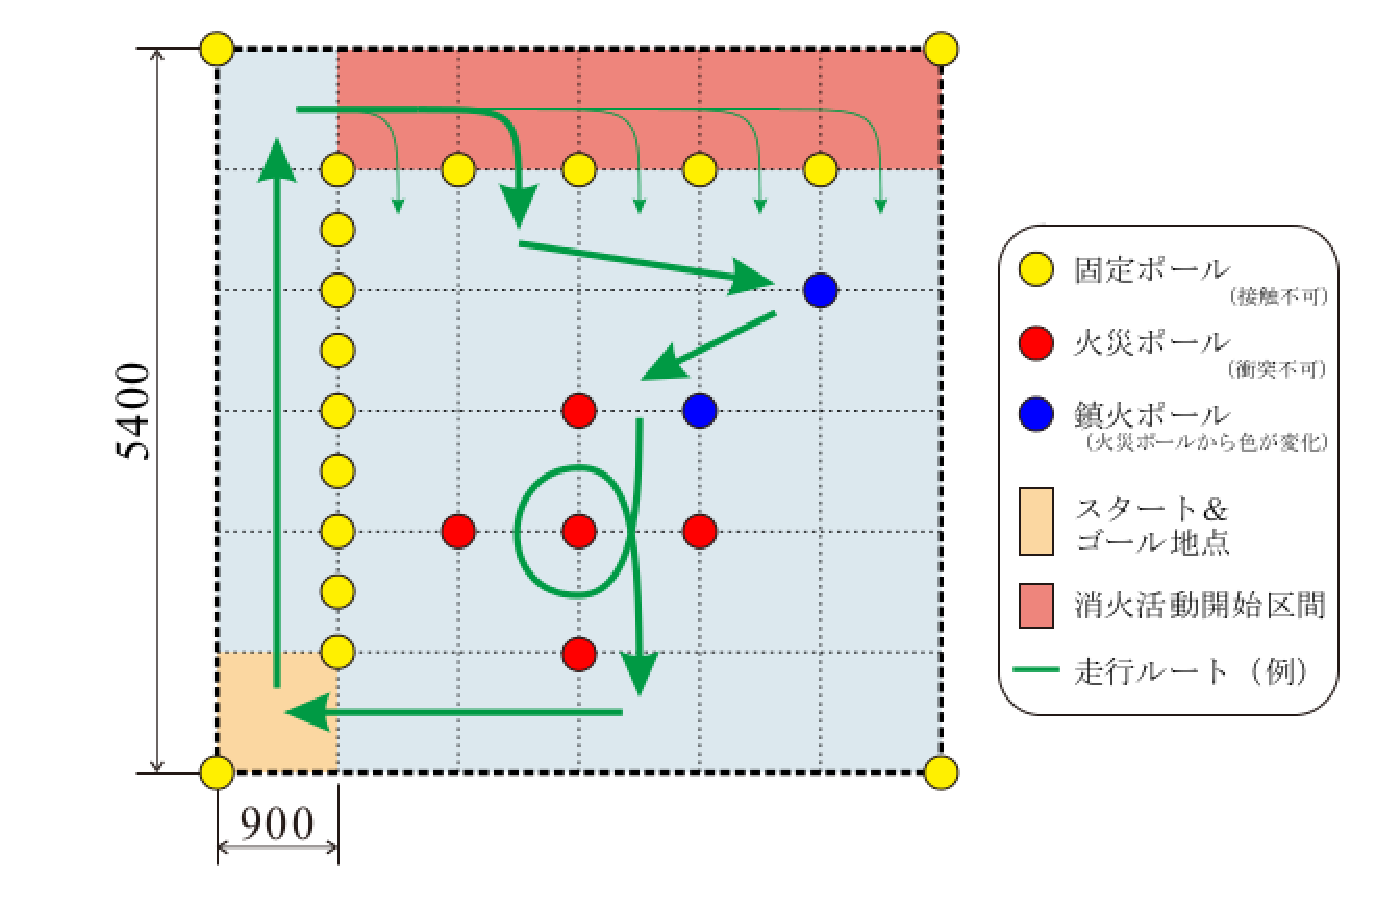
\includegraphics[width=1.0\hsize]{course.eps}
    \caption{2017年度 RCR走行コース}
    \label{course}
  \end{center}
\end{figure}


\newpage
\section{ロボットカーの設計コンセプト}
本年度のRCRでの我々の設計コンセプトは,

\section{消火方法}


\section{回路設計}


\end{document}
